%\documentstyle[epsfig]{article}
%\documentclass[a4paper, 11pt]{article}
%\documentclass[a4paper]{article}
\documentclass[]{book}
\usepackage[dvips]{epsfig,graphicx}
\usepackage{verbatim}
\usepackage{array}
\usepackage{color}
%\usepackage{colortbl}
\usepackage{longtable}
\usepackage{epsfig}
\usepackage{amsmath,amsfonts}
\pagestyle{myheadings}
\usepackage{latexsym}
\usepackage{graphicx}
\usepackage{longtable,dcolumn,multirow}
\usepackage{algorithm}
\usepackage{algorithmic}

\setlength\oddsidemargin{0.7in}
\setlength\evensidemargin{0.7in}

%\newcommand{\mb}[1]{B_{#1}}

\newtheorem{theo}{Theorem}
\newtheorem{defi}{Definition}
\newtheorem{Algo}{Algorithm}
\newtheorem{Remark}{Remark}
\newcommand{\alg}[1]{\Algo: {\rm {#1}}}


\newcommand {\h} {\hspace{2mm}}
\newcommand {\hh} {\hspace{5mm}}
\newcommand {\hhh} {\hspace{10mm}}

\let\cleardoublepage\clearpage

\title{\Huge{{\bf MAGMA}} Library\\
       {\begin{flushleft} 
         \hspace{25mm} {\large version 0.1}
        \end{flushleft}
       }\\
       {\begin{flushright}
          \vspace{-0.4in} 
          \line(1,0){3.7in}
        %\end{flushright}
        \\
        \vspace{0.4in} 
        \begin{minipage}[bottom]{3.7in}
          {\large
            S. Tomov \hh J. Dongarra \hh V. Volkov \hh  J. Demmel
          }
        \end{minipage}
        \end{flushright}
       }
      }


%\author{
% S. Tomov \\
% \and J. Dongarra
% \and J. Demmel
% \and V. Volkov
%}

%\institute{
% University of Tennessee (USA) \\
% \and
% Oak Ridge National Laboratory (USA) \\
% \and
% University of Manchester (UK)\\
%}
%\date{\today}
\date{}
\begin{document}

\maketitle
%\vskip 0.5cm
%\begin{center}
%{\large LAPACK Working Note 200}\\
%\end{center}
%\vskip 0.5cm

%\vskip 0.3cm
%\begin{center}
%{May 24, 2009}\\
%\end{center}
%\vskip 0.3cm

\vspace{2in}
\begin{verbatim}
    -- MAGMA (version 0.1) --
       Univ. of Tennessee, Knoxville
       Univ. of California, Berkeley
       Univ. of Colorado, Denver
       June 2009
\end{verbatim}


\vspace{0.2in}
\begin{verbatim}
       MAGMA project homepage: 
         http://icl.cs.utk.edu/magma/

       MAGMA project collaborators:
         M. Baboulin (U Coimbra, Portugal)
         J. Demmel   (UC Berkeley)
         J. Dongarra (UT Knoxville)
         J. Kurzak   (UT Knoxville)
         J. Langou   (UC Denver)
         S. Tomov    (UT Knoxville)
         V. Volkov   (UC Berkeley)
\end{verbatim}


%\begin{abstract}
% 
%\textbf{Keywords}:
%
%\end{abstract}

\tableofcontents

%%%%%%%%%%%%%%%%%%%%%%%%%%%%%%%%%%%%%%%%%%%%%%%%%%%%%%%%%%%%%%%%%%%%%%%%%%%%%%%
\chapter{The MAGMA Library}
%%%%%%%%%%%%%%%%%%%%%%%%%%%%%%%%%%%%%%%%%%%%%%%%%%%%%%%%%%%%%%%%%%%%%%%%%%%%%%%


{\bf MAGMA} stands for {\it Matrix Algebra for GPU and Multicore 
Architectures} and is the name of a project on the development of a 
dense linear algebra library similar to LAPACK but for 
heterogeneous/hybrid architectures, starting with current 
Multicore+GPU systems \cite{posterSC}. MAGMA's homepage is 

\vspace{0.05in}
\noindent
{\bf {\tt http://icl.cs.utk.edu/magma/}}
\vspace{0.1in}

The current release is intended for a single GPU and it's host 
-- see the specifications in Section \ref{hardware}.
MAGMA (version 0.1) includes the 3 one-sided matrix factorizations:
LU, QR, and Cholesky. There are functions for single and double precision 
arithmetic and for each of them there are 2 LAPACK-style interfaces. 
The first one, referred to as
{\bf CPU interface}, takes the input and produces the result in the CPU's
memory. The second, referred to as {\bf GPU interface}, 
takes the input and produces the result in the GPU's memory.

\vspace{0.1in}
The algorithm names are derived by the corresponding LAPACK names,
prefixed by {\tt magma\_}, and for the case of the GPU interface
suffixed by {\tt \_gpu}.

\vspace{0.1in}
This is an alpha release. It is based on the {\bf hybridization} of the
corresponding LAPACK algorithms \cite{lawn210,VolkovSC} and GPU motivated 
algorithmic innovations \cite{VolkovSC,posterSC}. The accuracy is as in LAPACK.
The performance relies on the performance of the CPU BLAS and GPU BLAS used. 
Upcoming releases will incorporate developments on 
\vspace{-0.05in}
\begin{itemize}
\item Auto-tuning \cite{lawn212}; \vspace{-0.05in}
\item Optimized GPU BLAS \cite{VolkovSC,lawn212}; \vspace{-0.05in}
\item New routines allowing for trade off   
      between performance and accuracy 
      (including mixed precision) \cite{posterSC,VolkovSC};
      \vspace{-0.05in} 
\item Routines for optimized use of the multicore host
      \cite{lawn210,lawn219}; \vspace{-0.05in}
\item Two-sided factorizations and eigen-problem solvers 
      \cite{lawn219}. \vspace{-0.05in}
\end{itemize}
A reference performance is given in Chapter \ref{ch:performance}. 


%%%%%%%%%%%%%%%%%%%%%%%%%%%%%%%%%%%%%%%%%%%%%%%%%%%%%%%%%%%%%%%%%%%%%%%%%%%%%%%
\newpage
\section{Function {\tt {\bf magma\_sgetrf}}}
%%%%%%%%%%%%%%%%%%%%%%%%%%%%%%%%%%%%%%%%%%%%%%%%%%%%%%%%%%%%%%%%%%%%%%%%%%%%%%%
\begin{verbatim}
int 
magma_sgetrf(int *m, int *n, float *a, int *lda, 
             int *ipiv, float *work, float *da, int *info)
{
/*  -- MAGMA (version 0.1) --
       Univ. of Tennessee, Knoxville
       Univ. of California, Berkeley
       Univ. of Colorado, Denver
       June 2009

    Purpose   
    =======   

    SGETRF computes an LU factorization of a general M-by-N matrix A   
    using partial pivoting with row interchanges.   

    The factorization has the form   
       A = P * L * U   
    where P is a permutation matrix, L is lower triangular with unit   
    diagonal elements (lower trapezoidal if m > n), and U is upper   
    triangular (upper trapezoidal if m < n).   

    This is the right-looking Level 3 BLAS version of the algorithm.   

    Arguments   
    =========   

    M       (input) INTEGER   
            The number of rows of the matrix A.  M >= 0.   

    N       (input) INTEGER   
            The number of columns of the matrix A.  N >= 0.   

    A       (input/output) REAL array, dimension (LDA,N)   
            On entry, the M-by-N matrix to be factored.   
            On exit, the factors L and U from the factorization   
            A = P*L*U; the unit diagonal elements of L are not stored.   

            Higher performance is achieved if A is in pinned memory, 
            e.g. allocated using cudaMallocHost.

    LDA     (input) INTEGER   
            The leading dimension of the array A.  LDA >= max(1,M).   

    IPIV    (output) INTEGER array, dimension (min(M,N))   
            The pivot indices; for 1 <= i <= min(M,N), row i of the   
            matrix was interchanged with row IPIV(i).   

    WORK    (workspace/output) REAL array, dimension >= N*NB,
            where NB can be obtained through magma_get_sgetrf_nb(M).

            Higher performance is achieved if WORK is in pinned memory, 
            e.g. allocated using cudaMallocHost.

    DA      (workspace)  REAL array on the GPU, dimension 
            (max(M, N)+ k1)^2 + (M + k2)*NB + 2*NB^2,
            where NB can be obtained through magma_get_sgetrf_nb(M).
            k1 < 32 and k2 < 32 are such that 
            (max(M, N) + k1)%32==0 and (M+k2)%32==0.

    INFO    (output) INTEGER   
            = 0:  successful exit   
            < 0:  if INFO = -i, the i-th argument had an illegal value   
            > 0:  if INFO = i, U(i,i) is exactly zero. The factorization   
                  has been completed, but the factor U is exactly   
                  singular, and division by zero will occur if it is used   
                  to solve a system of equations.   

    ===================================================================== */
\end{verbatim}

%%%%%%%%%%%%%%%%%%%%%%%%%%%%%%%%%%%%%%%%%%%%%%%%%%%%%%%%%%%%%%%%%%%%%%%%%%%%%%%
\newpage
\section{Function {\tt {\bf magma\_sgeqrf}}}
%%%%%%%%%%%%%%%%%%%%%%%%%%%%%%%%%%%%%%%%%%%%%%%%%%%%%%%%%%%%%%%%%%%%%%%%%%%%%%%
\begin{verbatim}
int 
magma_sgeqrf(int *m, int *n, float *a, int  *lda,  float  *tau,
             float *work, int *lwork, float *da, int *info )
{
/*  -- MAGMA (version 0.1) --
       Univ. of Tennessee, Knoxville
       Univ. of California, Berkeley
       Univ. of Colorado, Denver
       June 2009

    Purpose   
    =======   

    SGEQRF computes a QR factorization of a real M-by-N matrix A:   
    A = Q * R.   

    Arguments   
    =========   

    M       (input) INTEGER   
            The number of rows of the matrix A.  M >= 0.   

    N       (input) INTEGER   
            The number of columns of the matrix A.  N >= 0.   

    A       (input/output) REAL array, dimension (LDA,N)   
            On entry, the M-by-N matrix A.   
            On exit, the elements on and above the diagonal of the array   
            contain the min(M,N)-by-N upper trapezoidal matrix R (R is   
            upper triangular if m >= n); the elements below the diagonal,   
            with the array TAU, represent the orthogonal matrix Q as a   
            product of min(m,n) elementary reflectors (see Further   
            Details).   

            Higher performance is achieved if A is in pinned memory, 
            e.g. allocated using cudaMallocHost.

    LDA     (input) INTEGER   
            The leading dimension of the array A.  LDA >= max(1,M).   

    TAU     (output) REAL array, dimension (min(M,N))   
            The scalar factors of the elementary reflectors (see Further   
            Details).   

    WORK    (workspace/output) REAL array, dimension (MAX(1,LWORK))   
            On exit, if INFO = 0, WORK(1) returns the optimal LWORK.   

	    Higher performance is achieved if WORK is in pinned memory, 
            e.g. allocated using cudaMallocHost.

    LWORK   (input) INTEGER   
            The dimension of the array WORK.  LWORK >= N*NB, 
            where NB can be obtained through magma_get_sgeqrf_nb(M).   

            If LWORK = -1, then a workspace query is assumed; the routine   
            only calculates the optimal size of the WORK array, returns   
            this value as the first entry of the WORK array, and no error   
            message related to LWORK is issued.

    DA      (workspace)  REAL array on the GPU, dimension N*(M + NB), 
            where NB can be obtained through magma_get_sgeqrf_nb(M).
            (size to be reduced in upcoming versions).

    INFO    (output) INTEGER   
            = 0:  successful exit   
            < 0:  if INFO = -i, the i-th argument had an illegal value   

    Further Details   
    ===============   

    The matrix Q is represented as a product of elementary reflectors   

       Q = H(1) H(2) . . . H(k), where k = min(m,n).   

    Each H(i) has the form   

       H(i) = I - tau * v * v'   

    where tau is a real scalar, and v is a real vector with   
    v(1:i-1) = 0 and v(i) = 1; v(i+1:m) is stored on exit in A(i+1:m,i),   
    and tau in TAU(i).   

    ===================================================================== */
\end{verbatim}

%%%%%%%%%%%%%%%%%%%%%%%%%%%%%%%%%%%%%%%%%%%%%%%%%%%%%%%%%%%%%%%%%%%%%%%%%%%%%%%
\newpage
\section{Function {\tt {\bf magma\_spotrf}}}
%%%%%%%%%%%%%%%%%%%%%%%%%%%%%%%%%%%%%%%%%%%%%%%%%%%%%%%%%%%%%%%%%%%%%%%%%%%%%%%
\begin{verbatim}
int 
magma_spotrf(char *uplo, int *n, float *a, int *lda, float *work, 
             int *info)
{
/*  -- MAGMA (version 0.1) --
       Univ. of Tennessee, Knoxville
       Univ. of California, Berkeley
       Univ. of Colorado, Denver
       June 2009

    Purpose   
    =======   

    SPOTRF computes the Cholesky factorization of a real symmetric   
    positive definite matrix A.   

    The factorization has the form   
       A = U**T * U,  if UPLO = 'U', or   
       A = L  * L**T,  if UPLO = 'L',   
    where U is an upper triangular matrix and L is lower triangular.   

    This is the block version of the algorithm, calling Level 3 BLAS.   

    Arguments   
    =========   

    UPLO    (input) CHARACTER*1   
            = 'U':  Upper triangle of A is stored;   
            = 'L':  Lower triangle of A is stored.   

    N       (input) INTEGER   
            The order of the matrix A.  N >= 0.   

    A       (input/output) REAL array, dimension (LDA,N)   
            On entry, the symmetric matrix A.  If UPLO = 'U', the leading   
            N-by-N upper triangular part of A contains the upper   
            triangular part of the matrix A, and the strictly lower   
            triangular part of A is not referenced.  If UPLO = 'L', the   
            leading N-by-N lower triangular part of A contains the lower   
            triangular part of the matrix A, and the strictly upper   
            triangular part of A is not referenced.   

            On exit, if INFO = 0, the factor U or L from the Cholesky   
            factorization A = U**T*U or A = L*L**T.   

            Higher performance is achieved if A is in pinned memory, 
            e.g. allocated using cudaMallocHost.

    LDA     (input) INTEGER   
            The leading dimension of the array A.  LDA >= max(1,N).   

    WORK    (workspace) REAL array on the GPU, dimension (N, N)
            (size to be reduced in upcoming versions).

    INFO    (output) INTEGER   
            = 0:  successful exit   
            < 0:  if INFO = -i, the i-th argument had an illegal value   
            > 0:  if INFO = i, the leading minor of order i is not   
                  positive definite, and the factorization could not be   
                  completed.   

    ===================================================================== */
\end{verbatim}

%%%%%%%%%%%%%%%%%%%%%%%%%%%%%%%%%%%%%%%%%%%%%%%%%%%%%%%%%%%%%%%%%%%%%%%%%%%%%%%
\newpage
\section{Function {\tt {\bf magma\_sgetrf\_gpu}}}
%%%%%%%%%%%%%%%%%%%%%%%%%%%%%%%%%%%%%%%%%%%%%%%%%%%%%%%%%%%%%%%%%%%%%%%%%%%%%%%
\begin{verbatim}
int 
magma_sgetrf_gpu(int *m, int *n, float *a, int *lda, 
                 int *ipiv, float *work, int *info)
{
/*  -- MAGMA (version 0.1) --
       Univ. of Tennessee, Knoxville
       Univ. of California, Berkeley
       Univ. of Colorado, Denver
       June 2009

    Purpose   
    =======   

    SGETRF computes an LU factorization of a general M-by-N matrix A   
    using partial pivoting with row interchanges.   

    The factorization has the form   
       A = P * L * U   
    where P is a permutation matrix, L is lower triangular with unit   
    diagonal elements (lower trapezoidal if m > n), and U is upper   
    triangular (upper trapezoidal if m < n).   

    This is the right-looking Level 3 BLAS version of the algorithm.   

    Arguments   
    =========   

    M       (input) INTEGER   
            The number of rows of the matrix A.  M >= 0.   

    N       (input) INTEGER   
            The number of columns of the matrix A.  N >= 0.   

    A       (input/output) REAL array on the GPU, dimension (LDA,N) where
            LDA >= max(M, N)+k1 , k1<32 such that (max(M, N)+k1)%32==0.
            The memory pointed by A should be at least 
            (max(M, N) + k1)^2 + (M + k2)*NB + 2*NB^2
            where k2 < 32 such that (M + k2) %32 == 0.
                 
            On entry, the M-by-N matrix to be factored.   
            On exit, the factors L and U from the factorization   
            A = P*L*U; the unit diagonal elements of L are not stored.   
            The rest of A is considered work space and is changed.

    LDA     (input) INTEGER   
            The leading dimension of the array A.  LDA >= max(1,M).   

    IPIV    (output) INTEGER array, dimension (min(M,N))   
            The pivot indices; for 1 <= i <= min(M,N), row i of the   
            matrix was interchanged with row IPIV(i).   

    WORK    (workspace/output) REAL array, dimension >= N*NB,
            where NB can be obtained through magma_get_sgetrf_nb(M).

            Higher performance is achieved if WORK is in pinned memory, 
            e.g. allocated using cudaMallocHost.

    INFO    (output) INTEGER   
            = 0:  successful exit   
            < 0:  if INFO = -i, the i-th argument had an illegal value   
            > 0:  if INFO = i, U(i,i) is exactly zero. The factorization   
                  has been completed, but the factor U is exactly   
                  singular, and division by zero will occur if it is used   
                  to solve a system of equations.   

    ===================================================================== */
\end{verbatim}

%%%%%%%%%%%%%%%%%%%%%%%%%%%%%%%%%%%%%%%%%%%%%%%%%%%%%%%%%%%%%%%%%%%%%%%%%%%%%%%
\newpage
\section{Function {\tt {\bf magma\_sgeqrf\_gpu}}}
%%%%%%%%%%%%%%%%%%%%%%%%%%%%%%%%%%%%%%%%%%%%%%%%%%%%%%%%%%%%%%%%%%%%%%%%%%%%%%%
\begin{verbatim}
int 
magma_sgeqrf_gpu(int *m, int *n, float *a, int  *lda,  float  *tau,
                 float *work, int *lwork, float *dwork, int *info )
{
/*  -- MAGMA (version 0.1) --
       Univ. of Tennessee, Knoxville
       Univ. of California, Berkeley
       Univ. of Colorado, Denver
       June 2009

    Purpose   
    =======   

    SGEQRF computes a QR factorization of a real M-by-N matrix A:   
    A = Q * R.   

    Arguments   
    =========   

    M       (input) INTEGER   
            The number of rows of the matrix A.  M >= 0.   

    N       (input) INTEGER   
            The number of columns of the matrix A.  N >= 0.   

    A       (input/output) REAL array on the GPU, dimension (LDA,N)   
            On entry, the M-by-N matrix A.   
            On exit, the elements on and above the diagonal of the array   
            contain the min(M,N)-by-N upper trapezoidal matrix R (R is   
            upper triangular if m >= n); the elements below the diagonal,   
            with the array TAU, represent the orthogonal matrix Q as a   
            product of min(m,n) elementary reflectors (see Further   
            Details).

    LDA     (input) INTEGER   
            The leading dimension of the array A.  LDA >= max(1,M).   

    TAU     (output) REAL array, dimension (min(M,N))   
            The scalar factors of the elementary reflectors (see Further   
            Details).   

    WORK    (workspace/output) REAL array, dimension (MAX(1,LWORK))   
            On exit, if INFO = 0, WORK(1) returns the optimal LWORK.   

            Higher performance is achieved if A is in pinned memory, 
            e.g. allocated using cudaMallocHost.

    LWORK   (input) INTEGER   
            The dimension of the array WORK.  LWORK >= (M+N)*NB,   
            where NB can be obtained through magma_get_sgeqrf_nb(M).

            If LWORK = -1, then a workspace query is assumed; the routine   
            only calculates the optimal size of the WORK array, returns   
            this value as the first entry of the WORK array, and no error   
            message related to LWORK is issued.   

    DWORK   (workspace)  REAL array on the GPU, dimension N*NB,
            where NB can be obtained through magma_get_sgeqrf_nb(M).

    INFO    (output) INTEGER   
            = 0:  successful exit   
            < 0:  if INFO = -i, the i-th argument had an illegal value   

    Further Details   
    ===============   

    The matrix Q is represented as a product of elementary reflectors   

       Q = H(1) H(2) . . . H(k), where k = min(m,n).   

    Each H(i) has the form   

       H(i) = I - tau * v * v'   

    where tau is a real scalar, and v is a real vector with   
    v(1:i-1) = 0 and v(i) = 1; v(i+1:m) is stored on exit in A(i+1:m,i),   
    and tau in TAU(i).   

    ===================================================================== */
\end{verbatim}

%%%%%%%%%%%%%%%%%%%%%%%%%%%%%%%%%%%%%%%%%%%%%%%%%%%%%%%%%%%%%%%%%%%%%%%%%%%%%%%
\newpage
\section{Function {\tt {\bf magma\_spotrf\_gpu}}}
%%%%%%%%%%%%%%%%%%%%%%%%%%%%%%%%%%%%%%%%%%%%%%%%%%%%%%%%%%%%%%%%%%%%%%%%%%%%%%%
\begin{verbatim}
int 
magma_spotrf_gpu(char *uplo, int *n, float *a, int *lda, 
                 float *work, int *info)
{
/*  -- MAGMA (version 0.1) --
       Univ. of Tennessee, Knoxville
       Univ. of California, Berkeley
       Univ. of Colorado, Denver
       June 2009

    Purpose   
    =======   

    SPOTRF computes the Cholesky factorization of a real symmetric   
    positive definite matrix A.   

    The factorization has the form   
       A = U**T * U,  if UPLO = 'U', or   
       A = L  * L**T,  if UPLO = 'L',   
    where U is an upper triangular matrix and L is lower triangular.   

    This is the block version of the algorithm, calling Level 3 BLAS.   

    Arguments   
    =========   

    UPLO    (input) CHARACTER*1   
            = 'U':  Upper triangle of A is stored;   
            = 'L':  Lower triangle of A is stored.   

    N       (input) INTEGER   
            The order of the matrix A.  N >= 0.   

    A       (input/output) REAL array on the GPU, dimension (LDA,N)   
            On entry, the symmetric matrix A.  If UPLO = 'U', the leading   
            N-by-N upper triangular part of A contains the upper   
            triangular part of the matrix A, and the strictly lower   
            triangular part of A is not referenced.  If UPLO = 'L', the   
            leading N-by-N lower triangular part of A contains the lower   
            triangular part of the matrix A, and the strictly upper   
            triangular part of A is not referenced.   

            On exit, if INFO = 0, the factor U or L from the Cholesky   
            factorization A = U**T*U or A = L*L**T.   

    LDA     (input) INTEGER   
            The leading dimension of the array A.  LDA >= max(1,N).   

    WORK    (workspace) REAL array, dimension at least (nb, nb)
            where nb can be obtained through magma_get_spotrf_nb(*n)
            Work array allocated with cudaMallocHost.

    INFO    (output) INTEGER   
            = 0:  successful exit   
            < 0:  if INFO = -i, the i-th argument had an illegal value   
            > 0:  if INFO = i, the leading minor of order i is not   
                  positive definite, and the factorization could not be   
                  completed.   

    ===================================================================== */
\end{verbatim}

%%%%%%%%%%%%%%%%%%%%%%%%%%%%%%%%%%%%%%%%%%%%%%%%%%%%%%%%%%%%%%%%%%%%%%%%%%%%%%%
\newpage
\section{Function {\tt {\bf magma\_dgetrf}}}
%%%%%%%%%%%%%%%%%%%%%%%%%%%%%%%%%%%%%%%%%%%%%%%%%%%%%%%%%%%%%%%%%%%%%%%%%%%%%%%
\begin{verbatim}
int 
magma_dgetrf(int *m, int *n, double *a, int *lda, 
             int *ipiv, double *work, double *da, int *info)
{
/*  -- MAGMA (version 0.1) --
       Univ. of Tennessee, Knoxville
       Univ. of California, Berkeley
       Univ. of Colorado, Denver
       June 2009

    Purpose   
    =======   

    DGETRF computes an LU factorization of a general M-by-N matrix A   
    using partial pivoting with row interchanges.   

    The factorization has the form   
       A = P * L * U   
    where P is a permutation matrix, L is lower triangular with unit   
    diagonal elements (lower trapezoidal if m > n), and U is upper   
    triangular (upper trapezoidal if m < n).   

    This is the right-looking Level 3 BLAS version of the algorithm.   

    Arguments   
    =========   

    M       (input) INTEGER   
            The number of rows of the matrix A.  M >= 0.   

    N       (input) INTEGER   
            The number of columns of the matrix A.  N >= 0.   

    A       (input/output) DOUBLE array, dimension (LDA,N)   
            On entry, the M-by-N matrix to be factored.   
            On exit, the factors L and U from the factorization   
            A = P*L*U; the unit diagonal elements of L are not stored.   

            Higher performance is achieved if A is in pinned memory, 
            e.g. allocated using cudaMallocHost.

    LDA     (input) INTEGER   
            The leading dimension of the array A.  LDA >= max(1,M).   

    IPIV    (output) INTEGER array, dimension (min(M,N))   
            The pivot indices; for 1 <= i <= min(M,N), row i of the   
            matrix was interchanged with row IPIV(i).   

    WORK    (workspace/output) DOUBLE array, dimension >= N*NB,
            where NB can be obtained through magma_get_sgetrf_nb(M).

            Higher performance is achieved if WORK is in pinned memory, 
            e.g. allocated using cudaMallocHost.

    DA      (workspace)  DOUBLE array on the GPU, dimension 
            (max(M, N)+ k1)^2 + (M + k2)*NB + 2*NB^2,
            where NB can be obtained through magma_get_sgetrf_nb(M).
            k1 < 32 and k2 < 32 are such that 
            (max(M, N) + k1)%32==0 and (M+k2)%32==0.

    INFO    (output) INTEGER   
            = 0:  successful exit   
            < 0:  if INFO = -i, the i-th argument had an illegal value   
            > 0:  if INFO = i, U(i,i) is exactly zero. The factorization   
                  has been completed, but the factor U is exactly   
                  singular, and division by zero will occur if it is used   
                  to solve a system of equations.   

    ===================================================================== */
\end{verbatim}

%%%%%%%%%%%%%%%%%%%%%%%%%%%%%%%%%%%%%%%%%%%%%%%%%%%%%%%%%%%%%%%%%%%%%%%%%%%%%%%
\newpage
\section{Function {\tt {\bf magma\_dgeqrf}}}
%%%%%%%%%%%%%%%%%%%%%%%%%%%%%%%%%%%%%%%%%%%%%%%%%%%%%%%%%%%%%%%%%%%%%%%%%%%%%%%
\begin{verbatim}
int 
magma_dgeqrf(int *m, int *n, double *a, int  *lda,  double  *tau,
             double *work, int *lwork, double *da, int *info )
{
/*  -- MAGMA (version 0.1) --
       Univ. of Tennessee, Knoxville
       Univ. of California, Berkeley
       Univ. of Colorado, Denver
       June 2009

    Purpose   
    =======   

    DGEQRF computes a QR factorization of a real M-by-N matrix A:   
    A = Q * R.   

    Arguments   
    =========   

    M       (input) INTEGER   
            The number of rows of the matrix A.  M >= 0.   

    N       (input) INTEGER   
            The number of columns of the matrix A.  N >= 0.   

    A       (input/output) DOUBLE array, dimension (LDA,N)   
            On entry, the M-by-N matrix A.   
            On exit, the elements on and above the diagonal of the array   
            contain the min(M,N)-by-N upper trapezoidal matrix R (R is   
            upper triangular if m >= n); the elements below the diagonal,   
            with the array TAU, represent the orthogonal matrix Q as a   
            product of min(m,n) elementary reflectors (see Further   
            Details).   

            Higher performance is achieved if A is in pinned memory, 
            e.g. allocated using cudaMallocHost.

    LDA     (input) INTEGER   
            The leading dimension of the array A.  LDA >= max(1,M).   

    TAU     (output) DOUBLE array, dimension (min(M,N))   
            The scalar factors of the elementary reflectors (see Further   
            Details).   

    WORK    (workspace/output) DOUBLE array, dimension (MAX(1,LWORK))   
            On exit, if INFO = 0, WORK(1) returns the optimal LWORK.   

	    Higher performance is achieved if WORK is in pinned memory, 
            e.g. allocated using cudaMallocHost.

    LWORK   (input) INTEGER   
            The dimension of the array WORK.  LWORK >= N*NB, 
            where NB can be obtained through magma_get_dgeqrf_nb(M).   

            If LWORK = -1, then a workspace query is assumed; the routine   
            only calculates the optimal size of the WORK array, returns   
            this value as the first entry of the WORK array, and no error   
            message related to LWORK is issued.

    DA      (workspace)  DOUBLE array on the GPU, dimension N*(M + NB), 
            where NB can be obtained through magma_get_dgeqrf_nb(M).
            (size to be reduced in upcoming versions).

    INFO    (output) INTEGER   
            = 0:  successful exit   
            < 0:  if INFO = -i, the i-th argument had an illegal value   

    Further Details   
    ===============   

    The matrix Q is represented as a product of elementary reflectors   

       Q = H(1) H(2) . . . H(k), where k = min(m,n).   

    Each H(i) has the form   

       H(i) = I - tau * v * v'   

    where tau is a real scalar, and v is a real vector with   
    v(1:i-1) = 0 and v(i) = 1; v(i+1:m) is stored on exit in A(i+1:m,i),   
    and tau in TAU(i).   

    ===================================================================== */
\end{verbatim}

%%%%%%%%%%%%%%%%%%%%%%%%%%%%%%%%%%%%%%%%%%%%%%%%%%%%%%%%%%%%%%%%%%%%%%%%%%%%%%%
\newpage
\section{Function {\tt {\bf magma\_dpotrf}}}
%%%%%%%%%%%%%%%%%%%%%%%%%%%%%%%%%%%%%%%%%%%%%%%%%%%%%%%%%%%%%%%%%%%%%%%%%%%%%%%
\begin{verbatim}
int 
magma_dpotrf(char *uplo, int *n, double *a, int *lda, double *work, 
             int *info)
{
/*  -- MAGMA (version 0.1) --
       Univ. of Tennessee, Knoxville
       Univ. of California, Berkeley
       Univ. of Colorado, Denver
       June 2009

    Purpose   
    =======   

    DPOTRF computes the Cholesky factorization of a real symmetric   
    positive definite matrix A.   

    The factorization has the form   
       A = U**T * U,  if UPLO = 'U', or   
       A = L  * L**T,  if UPLO = 'L',   
    where U is an upper triangular matrix and L is lower triangular.   

    This is the block version of the algorithm, calling Level 3 BLAS.   

    Arguments   
    =========   

    UPLO    (input) CHARACTER*1   
            = 'U':  Upper triangle of A is stored;   
            = 'L':  Lower triangle of A is stored.   

    N       (input) INTEGER   
            The order of the matrix A.  N >= 0.   

    A       (input/output) DOUBLE array, dimension (LDA,N)   
            On entry, the symmetric matrix A.  If UPLO = 'U', the leading   
            N-by-N upper triangular part of A contains the upper   
            triangular part of the matrix A, and the strictly lower   
            triangular part of A is not referenced.  If UPLO = 'L', the   
            leading N-by-N lower triangular part of A contains the lower   
            triangular part of the matrix A, and the strictly upper   
            triangular part of A is not referenced.   

            On exit, if INFO = 0, the factor U or L from the Cholesky   
            factorization A = U**T*U or A = L*L**T.   

            Higher performance is achieved if A is in pinned memory,
            e.g. allocated using cudaMallocHost.

    LDA     (input) INTEGER   
            The leading dimension of the array A.  LDA >= max(1,N).   

    WORK    (workspace) DOUBLE array on the GPU, dimension (N, N)
            (size to be reduced in upcoming versions).

    INFO    (output) INTEGER   
            = 0:  successful exit   
            < 0:  if INFO = -i, the i-th argument had an illegal value   
            > 0:  if INFO = i, the leading minor of order i is not   
                  positive definite, and the factorization could not be   
                  completed.   

    ===================================================================== */
\end{verbatim}

%%%%%%%%%%%%%%%%%%%%%%%%%%%%%%%%%%%%%%%%%%%%%%%%%%%%%%%%%%%%%%%%%%%%%%%%%%%%%%%
\newpage
\section{Function {\tt {\bf magma\_dgetrf\_gpu}}}
%%%%%%%%%%%%%%%%%%%%%%%%%%%%%%%%%%%%%%%%%%%%%%%%%%%%%%%%%%%%%%%%%%%%%%%%%%%%%%%
\begin{verbatim}
int 
magma_dgetrf_gpu(int *m, int *n, double *a, int *lda, 
                 int *ipiv, double *work, int *info)
{
/*  -- MAGMA (version 0.1) --
       Univ. of Tennessee, Knoxville
       Univ. of California, Berkeley
       Univ. of Colorado, Denver
       June 2009

    Purpose   
    =======   

    DGETRF computes an LU factorization of a general M-by-N matrix A   
    using partial pivoting with row interchanges.   

    The factorization has the form   
       A = P * L * U   
    where P is a permutation matrix, L is lower triangular with unit   
    diagonal elements (lower trapezoidal if m > n), and U is upper   
    triangular (upper trapezoidal if m < n).   

    This is the right-looking Level 3 BLAS version of the algorithm.   

    Arguments   
    =========   

    M       (input) INTEGER   
            The number of rows of the matrix A.  M >= 0.   

    N       (input) INTEGER   
            The number of columns of the matrix A.  N >= 0.   

    A       (input/output) DOUBLE array on the GPU, dimension (LDA,N) where
            LDA >= max(M, N)+k1 , k1<32 such that (max(M, N)+k1)%32==0.
            The memory pointed by A should be at least 
            (max(M, N) + k1)^2 + (M + k2)*NB + 2*NB^2
            where k2 < 32 such that (M + k2) %32 == 0.
                 
            On entry, the M-by-N matrix to be factored.   
            On exit, the factors L and U from the factorization   
            A = P*L*U; the unit diagonal elements of L are not stored.   
            The rest of A is considered work space and is changed.

    LDA     (input) INTEGER   
            The leading dimension of the array A.  LDA >= max(1,M).   

    IPIV    (output) INTEGER array, dimension (min(M,N))   
            The pivot indices; for 1 <= i <= min(M,N), row i of the   
            matrix was interchanged with row IPIV(i).   

    WORK    (workspace/output) DOUBLE array, dimension >= N*NB,
            where NB can be obtained through magma_get_dgetrf_nb(M).

            Higher performance is achieved if WORK is in pinned memory, 
            e.g. allocated using cudaMallocHost.

    INFO    (output) INTEGER   
            = 0:  successful exit   
            < 0:  if INFO = -i, the i-th argument had an illegal value   
            > 0:  if INFO = i, U(i,i) is exactly zero. The factorization   
                  has been completed, but the factor U is exactly   
                  singular, and division by zero will occur if it is used   
                  to solve a system of equations.   

    ===================================================================== */
\end{verbatim}

%%%%%%%%%%%%%%%%%%%%%%%%%%%%%%%%%%%%%%%%%%%%%%%%%%%%%%%%%%%%%%%%%%%%%%%%%%%%%%%
\newpage
\section{Function {\tt {\bf magma\_dgeqrf\_gpu}}}
%%%%%%%%%%%%%%%%%%%%%%%%%%%%%%%%%%%%%%%%%%%%%%%%%%%%%%%%%%%%%%%%%%%%%%%%%%%%%%%
\begin{verbatim}
int 
magma_dgeqrf_gpu(int *m, int *n, double *a, int  *lda,  double  *tau,
                 double *work, int *lwork, double *dwork, int *info )
{
/*  -- MAGMA (version 0.1) --
       Univ. of Tennessee, Knoxville
       Univ. of California, Berkeley
       Univ. of Colorado, Denver
       June 2009

    Purpose   
    =======   

    DGEQRF computes a QR factorization of a real M-by-N matrix A:   
    A = Q * R.   

    Arguments   
    =========   

    M       (input) INTEGER   
            The number of rows of the matrix A.  M >= 0.   

    N       (input) INTEGER   
            The number of columns of the matrix A.  N >= 0.   

    A       (input/output) DOUBLE array on the GPU, dimension (LDA,N)   
            On entry, the M-by-N matrix A.   
            On exit, the elements on and above the diagonal of the array   
            contain the min(M,N)-by-N upper trapezoidal matrix R (R is   
            upper triangular if m >= n); the elements below the diagonal,   
            with the array TAU, represent the orthogonal matrix Q as a   
            product of min(m,n) elementary reflectors (see Further   
            Details).

    LDA     (input) INTEGER   
            The leading dimension of the array A.  LDA >= max(1,M).   

    TAU     (output) DOUBLE array, dimension (min(M,N))   
            The scalar factors of the elementary reflectors (see Further   
            Details).   

    WORK    (workspace/output) DOUBLE array, dimension (MAX(1,LWORK))   
            On exit, if INFO = 0, WORK(1) returns the optimal LWORK.   

            Higher performance is achieved if A is in pinned memory, 
            e.g. allocated using cudaMallocHost.

    LWORK   (input) INTEGER   
            The dimension of the array WORK.  LWORK >= (M+N)*NB,   
            where NB can be obtained through magma_get_dgeqrf_nb(M).

            If LWORK = -1, then a workspace query is assumed; the routine   
            only calculates the optimal size of the WORK array, returns   
            this value as the first entry of the WORK array, and no error   
            message related to LWORK is issued.   

    DWORK   (workspace)  DOUBLE array on the GPU, dimension N*NB,
            where NB can be obtained through magma_get_dgeqrf_nb(M).

    INFO    (output) INTEGER   
            = 0:  successful exit   
            < 0:  if INFO = -i, the i-th argument had an illegal value   

    Further Details   
    ===============   

    The matrix Q is represented as a product of elementary reflectors   

       Q = H(1) H(2) . . . H(k), where k = min(m,n).   

    Each H(i) has the form   

       H(i) = I - tau * v * v'   

    where tau is a real scalar, and v is a real vector with   
    v(1:i-1) = 0 and v(i) = 1; v(i+1:m) is stored on exit in A(i+1:m,i),   
    and tau in TAU(i).   

    ===================================================================== */
\end{verbatim}

%%%%%%%%%%%%%%%%%%%%%%%%%%%%%%%%%%%%%%%%%%%%%%%%%%%%%%%%%%%%%%%%%%%%%%%%%%%%%%%
\newpage
\section{Function {\tt {\bf magma\_dpotrf\_gpu}}}
%%%%%%%%%%%%%%%%%%%%%%%%%%%%%%%%%%%%%%%%%%%%%%%%%%%%%%%%%%%%%%%%%%%%%%%%%%%%%%%
\begin{verbatim}
int 
magma_dpotrf_gpu(char *uplo, int *n, double *a, int *lda, double *work, 
                 int *info)
{
/*  -- MAGMA (version 0.1) --
       Univ. of Tennessee, Knoxville
       Univ. of California, Berkeley
       Univ. of Colorado, Denver
       June 2009

    Purpose   
    =======   

    DPOTRF computes the Cholesky factorization of a real symmetric   
    positive definite matrix A.   

    The factorization has the form   
       A = U**T * U,  if UPLO = 'U', or   
       A = L  * L**T,  if UPLO = 'L',   
    where U is an upper triangular matrix and L is lower triangular.   

    This is the block version of the algorithm, calling Level 3 BLAS.   

    Arguments   
    =========   

    UPLO    (input) CHARACTER*1   
            = 'U':  Upper triangle of A is stored;   
            = 'L':  Lower triangle of A is stored.   

    N       (input) INTEGER   
            The order of the matrix A.  N >= 0.   

    A       (input/output) DOUBLE array on the GPU, dimension (LDA,N)   
            On entry, the symmetric matrix A.  If UPLO = 'U', the leading   
            N-by-N upper triangular part of A contains the upper   
            triangular part of the matrix A, and the strictly lower   
            triangular part of A is not referenced.  If UPLO = 'L', the   
            leading N-by-N lower triangular part of A contains the lower   
            triangular part of the matrix A, and the strictly upper   
            triangular part of A is not referenced.   

            On exit, if INFO = 0, the factor U or L from the Cholesky   
            factorization A = U**T*U or A = L*L**T.   

    LDA     (input) INTEGER   
            The leading dimension of the array A.  LDA >= max(1,N).   

    WORK    (workspace) DOUBLE array, dimension at least (nb, nb)
            where nb can be obtained through magma_get_dpotrf_nb(*n)
            Work array allocated with cudaMallocHost.

    INFO    (output) INTEGER   
            = 0:  successful exit   
            < 0:  if INFO = -i, the i-th argument had an illegal value   
            > 0:  if INFO = i, the leading minor of order i is not   
                  positive definite, and the factorization could not be   
                  completed.   

    ===================================================================== */
\end{verbatim}


%%%%%%%%%%%%%%%%%%%%%%%%%%%%%%%%%%%%%%%%%%%%%%%%%%%%%%%%%%%%%%%%%%%%%%%%%%%%%%%
\chapter{Use}\label{ch:use}
%%%%%%%%%%%%%%%%%%%%%%%%%%%%%%%%%%%%%%%%%%%%%%%%%%%%%%%%%%%%%%%%%%%%%%%%%%%%%%%

%%%%%%%%%%%%%%%%%%%%%%%%%%%%%%%%%%%%%%%%%%%%%%%%%%%%%%%%%%%%%%%%%%%%%%%%%%%%%%%
\section{Hardware specifications}\label{hardware}
%%%%%%%%%%%%%%%%%%%%%%%%%%%%%%%%%%%%%%%%%%%%%%%%%%%%%%%%%%%%%%%%%%%%%%%%%%%%%%%
MAGMA version 0.1 is intended for a single CUDA enabled NVIDIA GPU and 
it's host. CUDA enabled GPUs are for example the GeForce 8 Series, 
the Tesla GPUs, and some Quadro GPUs \cite{GPUManual}. MAGMA's double 
precision routines can be used on CUDA enabled GPUs that support double 
precision arithmetic. 
These are for example the GeForce 200 Series and the Tesla solutions.
The host can be any shared memory multiprocessor for which LAPACK is 
suitable. One host core is required and multiple can be used through
multicore LAPACK implementation.

\vspace{0.2in}
%%%%%%%%%%%%%%%%%%%%%%%%%%%%%%%%%%%%%%%%%%%%%%%%%%%%%%%%%%%%%%%%%%%%%%%%%%%%%%%
\section{Software specifications}
%%%%%%%%%%%%%%%%%%%%%%%%%%%%%%%%%%%%%%%%%%%%%%%%%%%%%%%%%%%%%%%%%%%%%%%%%%%%%%%
MAGMA version 0.1 is a Linux release that requires
\begin{itemize}
  \item the CUDA driver, CUDA toolkit, and CUDA SDK
        \footnote{freely available from NVIDIA\\
                \hhh  http://www.nvidia.com/object/cuda\_get.html};
  \item CPU BLAS and LAPACK.
\end{itemize}

MAGMA users do not have to know CUDA in order to use the library. 
A testing directory gives examples on how to use every function (see Section 
\ref{testing}). Applications can use the CPU interface without any 
significant change to the application -- LAPACK calls have to be prefixed with
{\tt magma\_} and a workspace argument (for the GPU memory) has to be 
added (shown in the examples).

\newpage

%%%%%%%%%%%%%%%%%%%%%%%%%%%%%%%%%%%%%%%%%%%%%%%%%%%%%%%%%%%%%%%%%%%%%%%%%%%%%%%
\section{Testing}\label{testing}
%%%%%%%%%%%%%%%%%%%%%%%%%%%%%%%%%%%%%%%%%%%%%%%%%%%%%%%%%%%%%%%%%%%%%%%%%%%%%%%
Directory {\tt magma/testing} has drivers that test and show how
to use every function of this distribution. Below is an example
showing the output of the {\tt sgetrf} driver.

\begin{verbatim}
> ./testing_sgetrf
Using device 0: GeForce GTX 280

Usage: 
  testing_sgetrf -N 1024

  N    CPU GFlop/s    GPU GFlop/s    ||PA-LU|| / (||A||*N)
==========================================================
 1024     33.26          42.77         1.861593e-09
 2048     52.29          96.06         1.722339e-09
 3072     64.03         146.33         1.411851e-09
 4032     80.60         195.44         1.371482e-09
 5184     86.65         224.92         1.332554e-09
 6016     91.66         240.33         1.331916e-09
 7040     96.02         255.51         1.306940e-09
 8064     99.88         267.17         1.391934e-09
 9088    101.18         276.59         1.549758e-09
10112    104.38         284.30         1.661756e-09

\end{verbatim}

Performance and accuracy for particular values of the matrix
size can also be tested. Note that performance is slower
for sizes not divisible by certain powers of 2, e.g. 32, 64, etc. 
This issue will be addressed in future MAGMA releases (currently due
to CUBLAS being slower for those cases).

\begin{verbatim}
> ./testing_sgetrf -N 1026
Using device 0: GeForce GTX 280


  N    CPU GFlop/s    GPU GFlop/s    ||PA-LU|| / (||A||*N)
==========================================================
 1026     32.93          41.09         1.834303e-09
\end{verbatim}

%%%%%%%%%%%%%%%%%%%%%%%%%%%%%%%%%%%%%%%%%%%%%%%%%%%%%%%%%%%%%%%%%%%%%%%%%%%%%%%
\chapter{Performance}\label{ch:performance}

Here we give the reference performance results using MAGMA version 0.1 
in the following hardware and software configuration:

\vspace{0.2in}
\begin{description}
\item[GPU:]  NVIDIA GeForce GTX 280;
\item[CPU:] Intel Xeon dual socket quad-core @ 2.33 GHz;
\item[GPU BLAS:] CUBLAS 2.1;
\item[CPU BLAS:] MKL 10.0;
\item[Compiler:] gcc 4.1.2;
\item[Tuning:] Hand tuned (and hard coded).
\end{description}

\vspace{0.2in}
Note that this release is hand tuned for this particular configuration.
Different configurations may require different tuning in which case
there would be a negative impact on the performance.
Future releases will be auto-tuned using an empirically-based 
approach \cite{lawn212}. A handle to user tuning is given in file \\
{\tt magma/src/auxiliary.cpp} \\
through functions \\
{\tt magma\_get\_\{function name\}\_nb}\\
which, based on matrix
size, returns a block size to be used by the corresponding function.
Optimal sizes (for the functions in this distribution) 
would be a multiple of 32.

\newpage
%%%%%%%%%%%%%%%%%%%%%%%%%%%%%%%%%%%%%%%%%%%%%%%%%%%%%%%%%%%%%%%%%%%%%%%%%%%%%%%
\section{Single precision}

       \begin{figure}[!ht]
          \centering
          \hspace{-5mm}
          \includegraphics[angle=-90,scale=0.7]{sp-cpu.ps}
          %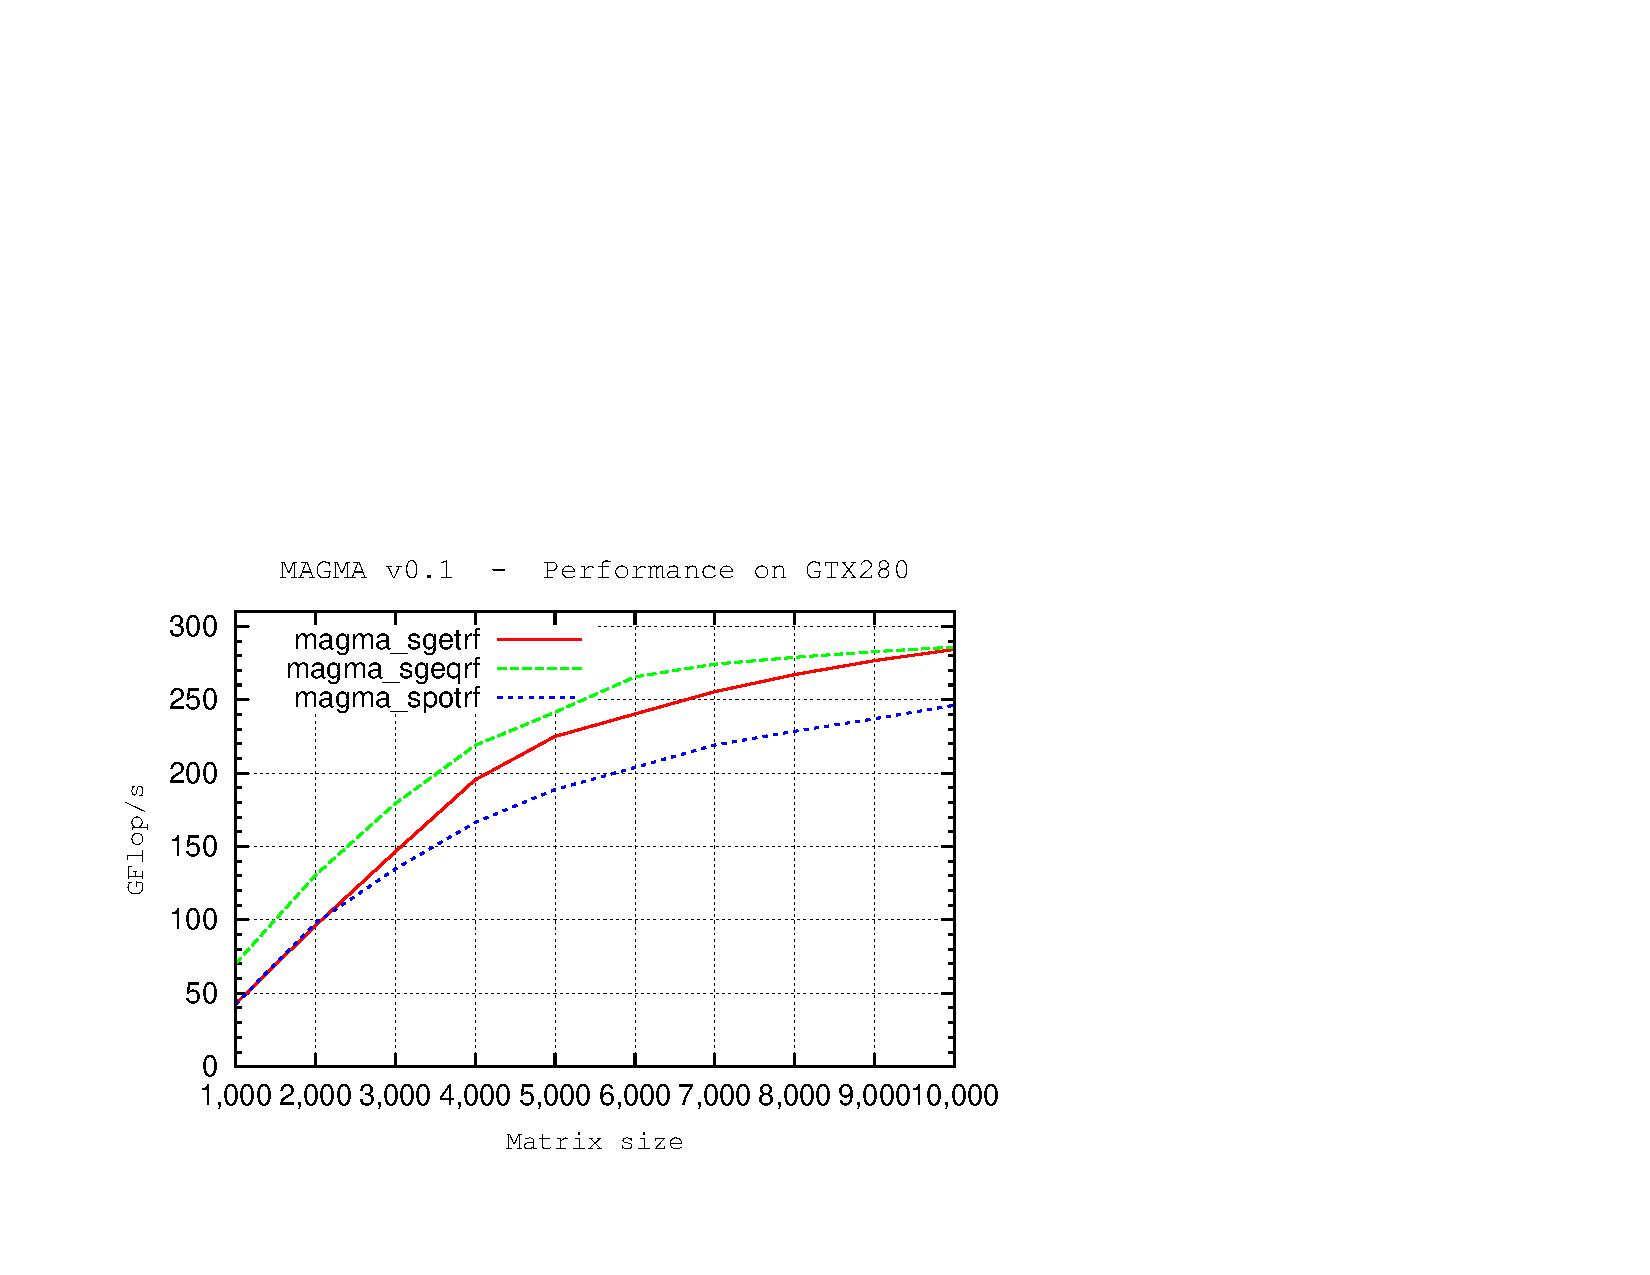
\includegraphics[width=7in]{sp-cpu.pdf}
          \caption{Performance of the {\bf CPU interface} 
                   one-sided factorizations.}
       \label{sp-cpu-performance}
       \end{figure}

       \begin{figure}[!ht]
          \centering
          \hspace{-5mm}
          \includegraphics[angle=-90,scale=0.7]{sp-gpu.ps}
          %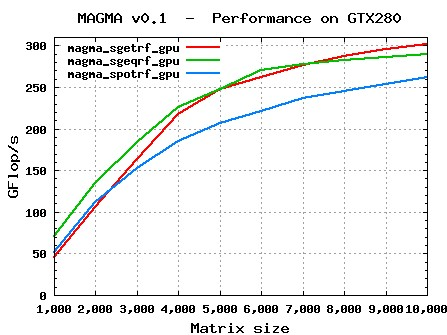
\includegraphics[width=5in]{sp-gpu.jpg}
          \caption{Performance of the {\bf GPU interface}
                   one-sided factorizations.}
       \label{sp-gpu-performance}
       \end{figure}
\newpage
\section{Double precision}

       \begin{figure}[!ht]
          \centering
          \hspace{-5mm}
          \includegraphics[angle=-90,scale=0.7]{dp-cpu.ps}
          %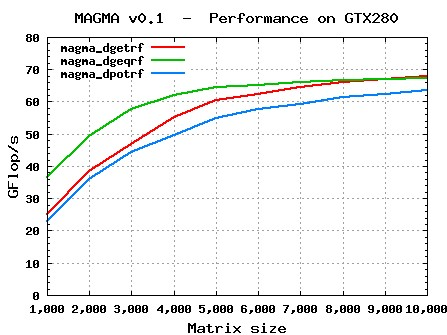
\includegraphics[width=5in]{dp-cpu.jpg}
          \caption{Performance of the {\bf CPU interface} 
                   one-sided factorizations.}
       \label{dp-cpu-performance}
       \end{figure}

       \begin{figure}[!ht]
          \centering
          \hspace{-5mm}
          \includegraphics[angle=-90,scale=0.7]{dp-gpu.ps}
          %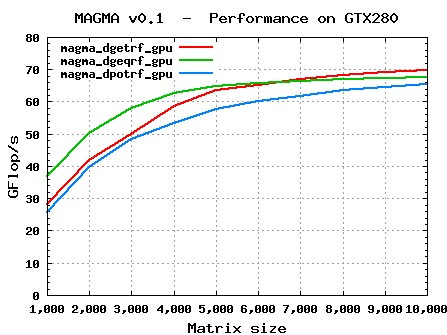
\includegraphics[width=5in]{dp-gpu.jpg}
          \caption{Performance of the {\bf GPU interface} 
                   one-sided factorizations.}
       \label{dp-gpu-performance}
       \end{figure}

%%%%%%%%%%%%%%%%%%%%%%%%%%%%%%%%%%%%%%%%%%%%%%%%%%%%%%%%%%%%%%%%%%%%%%%%%%%%%%%
%\addcontentsline{toc}{chapter}{Contributors}
%\chapter*{Contributors}

%%%%%%%%%%%%%%%%%%%%%%%%%%%%%%%%%%%%%%%%%%%%%%%%%%%%%%%%%%%%%%%%%%%%%%%%%%%%%%%


%%%%%%%%%%%%%%%%%%%%%%%%%%%%%%%%%%%%%%%%%%%%%%%%%%%%%%%%%%%%%%%%%%%%%%%%%%%%%%%
%\ackname{
\addcontentsline{toc}{chapter}{Acknowledgments}
\chapter*{Acknowledgments}
%{\bf Acknowledgments}.
This work is supported by Microsoft, the U.S. National Science Foundation,
and the U.S. Department of Energy. We thank NVIDIA and NVIDIA's Professor 
Partnership Program for their hardware donations.

%%%%%%%%%%%%%%%%%%%%%%%%%%%%%%%%%%%%%%%%%%%%%%%%%%%%%%%%%%%%%%%%%%%%%%%%%%%%%%%

\addcontentsline{toc}{chapter}{Bibliography}
\bibliographystyle{amsplain}
\bibliography{biblio}

\end{document}

set fichier=algochol
xfig -specialtext -latexfont -startlatexFont default $fichier.fig
fig2dev -L pstex $fichier.fig > $fichier.ps ; fig2dev -L pstex_t -p $fichier.ps $fichier.fig > $fichier.tex

%%%%%%%%%%%%%%%%%%%%%%%%%%%%%%%%%%%%%%%%%%%%%%%%%%%%%%%%%%%%%%%%%%%%%%%%%%%%%%%
